\LARGE{ \textbf {Лекция №1}}

Системы счисления - способ выражения и обозначения чисел по средствам некоторого
алфавита цифр.
Цифры - ограниченный набор символов (алфавит).\\
Позиционные и непозиционные системы счисления.

Непозиционные - такие, в которых значение цифры не завсит от её положения в числе. (Римская, наличные деньги)

Позиционные - такие, в которых значение цифры завсит от её положения в числе.

Основание С.С. - количество различных цифр, которое употребляется в позиционной С.С.
$$ N_b=a_{q_1}\cdot b^{q-1} + a_{q_2} \cdot b^{q-2} \cdots a_{q_0}\cdot b^0 + a_{q_{-1}}\cdot b^{-1},$$
\begin{equation}
   \sum_{i = -p}^{q-1} a_i b^i
\end{equation}
\begin{center}
  $ b>1 ; \quad b \in \mathbb{Z} $ \\
  $ a_i \in \mathbb{Z} \quad 0 \le a_i < b $ \\
\end{center}
 где $a_0 \cdots a_{n-1}  $ - цифры,\\
 $q$ - количество цифр в целой части,\\
 $p$ - в дробной, а $b$ - основание системы счисления.\\
 $ a_{q-1} $ - cтарший разряд числа.\\
 $ a_{-p} $ - младший разряд числа.\\

 \Large{ \textbf {Компактное представление чисел}}

Пусть существует некоторое $n$- разрядное устройство, которое может хранить числа.
\begin{itemize}
  \item $ b=2 \qquad n=12 \qquad W=24 \quad 2^n = 2^12 = 4096 $
  \item $ b=3 \qquad n=8 \qquad W=24 \quad 3^n = 3^8 = 6561 $
  \item $ b=10 \qquad n=4 \qquad W=10 \cdot 3 + 7 = 37 \quad $ - для числа ~6561
\end{itemize}

Это доказывает, что оптимальная $b = \ell \equiv 2.7 \quad b = 2 $, так как построить устройство с двумя состояниями проще, они надежнее.
\newpage

\Large{ \textbf {Преобразование чисел в различные С.С.}}
\begin{flalign*}
&(N)_{b_1} \\
&(N)_{b_2} - ? \\
&(N)_{b_2} = a_k \cdot b_2^k + a_{k-1} \cdot b_2^{k-1} + \cdots + a_1 b_2^1 + a_0 b_2^0 = \\
&= ( \cdots ((a_k \cdot b_2  + a_k-1)\cdot b_2 + a_k-2)\cdot b_2  + \cdots a_1) b_2 +a_0
\end{flalign*}

Если разделить на $b_2$, то получим новый младший разряд и остаток.
$$ (1101001)_2 = 64 + 32 + 8 + 1 = 105 $$

\Large{ \textbf {Перевод правильных дробей }}
\begin{flalign*}
&(N)_{b_1} \rightarrow
(?)_{b_2} \\
&(N)_{b_2} = C_{-1} \cdot b_2^{-1} + C_{-2} \cdot b_2^{-2} + C_k \cdot b^{-k}
\end{flalign*}

Повторяя $k$ раз получим $k$ цифр дробной части.\\
$
(0,625)_10 = (?)_2 = (0,101)_2 \\
$
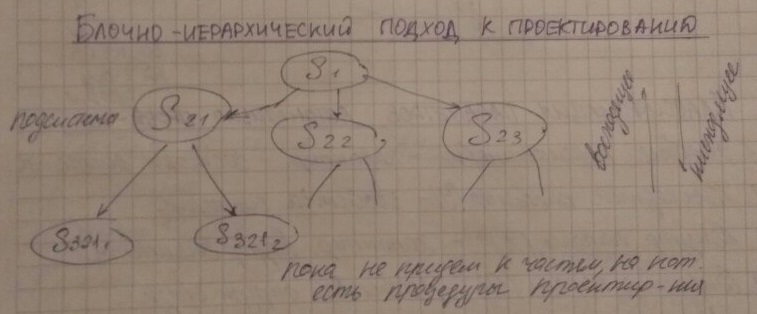
\includegraphics[width=\linewidth]{1}
Данный пример специально подобран , в смысле остаток равен 0 , процесс преобразования завершился на 3 итерации , в общем случае процесс преобразования может длится бесконечно. Процесс прерывают, когда заполнены все разряды разрядной сетки, либо при достижении нужной точности.
Если дробь смешанная то отдельно переводят целую часть числа, и отдельно дробную.
